\begin{figure}[tb]
  \begin{center}
    \scalebox{0.8}{%
      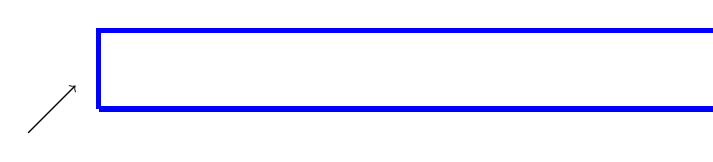
\begin{tikzpicture}
        \creategridjps{10}{3}
        \drawobstaclejps{4}{1}
        \drawobstaclejps{5}{1}
        \drawobstaclejps{7}{2}
%        \drawobstaclejps{7}{4}
%        \drawobstaclejps{6}{4}
%        \drawobstaclejps{3}{7}
%        \drawobstaclejps{2}{2}
%        \drawobstaclejps{3}{2}
        \draw[->] (0.7,0.7) -- (1.3,1.3);
        \drawgridnodejps{2}{2}{$N$}
        \drawgridnodejps{1}{1}{$P$}
%        \drawgridnodejps{7}{5}{$Z$}
        \drawgridnodejps{3}{2}{{\color{red} 1}}
        \drawgridnodejps{2}{1}{{\color{red} 2}}
        \drawgridnodejps{2}{3}{{\color{red} 3}}
        \drawgridnodejps{4}{2}{{\color{red} 4}}
        \drawgridnodejps{3}{1}{{\color{red} 5}}
        \drawgridnodejps{3}{3}{{\color{red} 6}}
        \drawgridnodejps{5}{2}{{\color{red} 7}}
        \drawgridnodejps{4}{1}{{\color{red} 8}}
        \drawgridnodejps{4}{3}{{\color{red} 9}}
        \draw[blue,line width=2pt] (1,1) -- (9,1) -- (9,2) -- (1,2) -- (1,1);
      \end{tikzpicture}%
    }
  \end{center}
\vspace{-1em}
  \caption[Example of block-based jumping]
{ \small
A current search state (the grid is assumed larger than the part presented).
The red numbers show in which order the traversability of the nodes is tested.
The blue rectangle represents the byte that is returned when we scan the
grid to read the value of location $N = \langle 2, 2\rangle$.
}
  \label{fig::jps2::gridforblocks}
\end{figure}
